\section{Master's Project: Design Decisions}

\subsection{Initial Plan}
Despite the many areas of improvement for our senior project, we initially believed that a functional tester was adequate for most student-designed VLSI chips. It is worth noting that at the time of our senior project semester, students in VLSI designed their chips using a 0.6 micron process. Generally, chips fabricated using this process cannot run beyond 25 MHz. As such, we believed the best course of action was to polish our system (e.g. simplify the user interface and setup) in order to allow students to test their chips' functionality. For any timing-sensitive chips, students would be advised to construct a development board for their chip and use a logic analyzer or oscilloscope to analyze signals in detail.

When we first proposed expanding upon our senior project for our Master's project, our basic plan was to do the following: 
\begin{itemize}
\item Eliminate the Numato Saturn and fabricate a MOSIS chip containing the finite state machine logic originally used by the Saturn.
\item Replace the double-buffered shift registers inside the Saturn with external double-buffered shift registers controlled by a MOSIS chip.
\item Implement autoschmooing by replacing the trimpot on our variable voltage regulator with a digital pot.
\item Expand upon our C Sharp program (e.g. create schmooing plots).
\item Try to redesign our main PCB with equilibrium tracing.
\end{itemize}

While the plan seemed solid at first, we quickly became concerned that the project may not have been challenging enough for a Master's project. We soon came to believe that attempting to implement both autoschmooing and real-time testing would provide a more suitable challenge to us, and so, we decided to revamp our entire senior project design.

\subsection{Revised Plan}
We redefined the goals of our Master's project as follows: 
\begin{itemize}
\item Simpler interface and setup. Ideally, the entire system would be plug-and-play.
\item Real-time testing (where a test cycle is executed immediately following completion of the preceding test cycle).
\item Timing information (via PCB equilibrium tracing).
\item Automated schmooing.
\item More test cycle configurations.
\end{itemize}

We spent Fall 2015 brainstorming ideas to implement the above goals. We proposed the schematic in Figure \ref{fig:f15_schematic} at the end of the semester. Below, we detail each major component of this schematic.

\begin{figure}
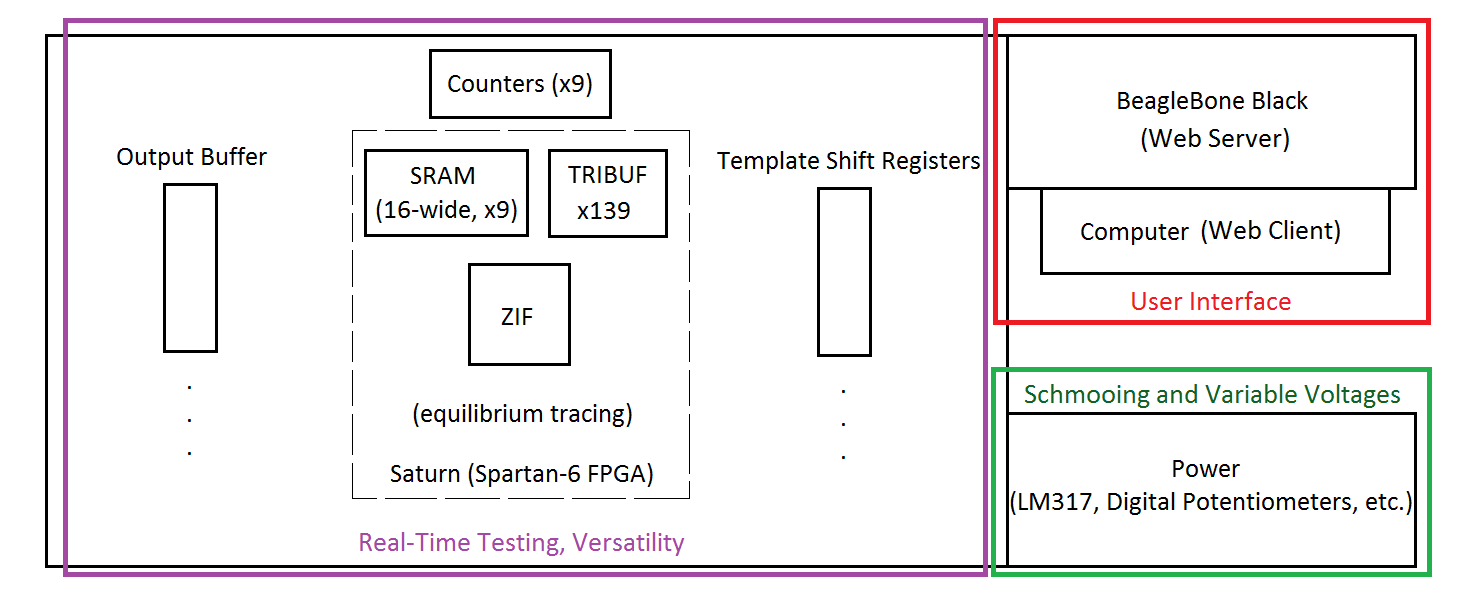
\includegraphics[width=1.0\textwidth]{original_schematic.png}
\caption{Schematic proposed at end of Fall 2015 semester.}
\label{fig:f15_schematic}
\end{figure}

\subsubsection{User Interface: BeagleBone Black Web Server}
TODO: Norm

\subsubsection{Reuse of Numato Saturn}
TODO: Daniel

\subsubsection{Real-Time Testing}
TODO: Norm, Daniel

\subsubsection{Automated Schmooing}
TODO: Daniel

\subsubsection{Timing Characteristics}
TODO: Norm, Daniel

\subsubsection{Modular Design}
TODO: Norm, Daniel

\newpage